\section*{پاسخ:}

تعداد کل بسته‌هایی که باید ارسال شود برابر است با: 
\(\frac{5000}{4}=1250\)


\begin{enumerate}
\begin{enumerate}
  \item در این روش پس از \lr{handshake} بستهٔ اول ارسال می‌شود. طبق صورت سؤال این بسته گم می‌شود و تأیید آن به میزبان B نمی‌رسد. پس از یک \lr{timeout} بستهٔ اول دوباره ارسال می‌شود و پس از آن در هر \lr{RTT} یک بسته توسط میزبان A دریافت و تایید آن به B می‌رسد. در نتیجه در کل طول می‌کشد تا میزبان B از دریافت کامل فایل اطمینان حاصل کند.
  \begin{flushleft}
  \text{\(1\,\text{\lr{Timeout}}+1250\,\text{\lr{RTT}}=1254\,\text{\lr{RTT}}\)}
  \end{flushleft}

  \item در این روش ابتدا میزبان B با توجه به اندازهٔ پنجرهٔ ارسال، سه بسته را ارسال می‌کند و پس از رخ دادن \lr{timeout} با وجود این‌که بسته‌های دوم و سوم گم نشده است هر سه بسته را دوباره ارسال می‌کند. پس از آن با صرف نظر کردن از زمان پردازش بسته‌ها، در هر \lr{RTT} سه بسته توسط میزبان A دریافت و تأیید آن‌ها به B می‌رسد. در نتیجه زمان کل برابر است با
\begin{flushleft}
\text{\(1\,\text{\lr{Timeout}}+\lceil1250/3\rceil\,\text{\lr{RTT}}=4+417=421\,\text{\lr{RTT}}\)}\\
 \end{flushleft}
  
  \item در این روش میزبان B سه بسته را ارسال می‌کند و پس از رخ دادن \lr{timeout} فقط بستهٔ اول را دوباره ارسال می‌کند. اما چون اندازهٔ پنجرهٔ ارسال برابر سه است و تأیید اولین بسته دریافت نشده نمی‌تواند بستهٔ جدیدی ارسال کند. پس از یک \lr{RTT} تأیید بستهٔ اول به B می‌رسد. تأییدهای بستهٔ دوم و سوم نیز پیش از این به B رسیده است. در نتیجه سه بستهٔ بعدی را ارسال می‌کند و از آن به بعد در هر \lr{RTT} سه بسته توسط میزبان A دریافت و تأیید آن‌ها به B می‌رسد. زمان کل برابر است با
  \begin{flushleft}
  \text{\(1\,\text{\lr{Timeout}}+1\,\text{\lr{RTT}}+\lceil1247/3\rceil\,\text{\lr{RTT}}=4+1+416=421\,\text{\lr{RTT}}\)}
\end{flushleft}
  
  \item این قسمت مشابه قسمت قبل خواهد بود با این تفاوت که اندازهٔ پنجرهٔ ارسال پنج است و در نتیجه میزبان پنج بسته را ارسال می‌کند. زمان کل برابر با مقدار زیر خواهد بود:
\begin{flushleft}
  \text{\(1\,\text{\lr{Timeout}}+1\,\text{\lr{RTT}}+\lceil1245/5\rceil\,\text{\lr{RTT}}=4+1+249=254\,\text{\lr{RTT}}\)}
\end{flushleft}

\end{enumerate}
\end{enumerate}

در شکل زیر می‌توانید نمودار ارسال برای نسخهٔ کوچک‌شدهٔ مسئله را ببینید. میزبان B قصد ارسال ۵ بسته به میزبان A دارد و برای سادگی فرض شده است که اندازهٔ هر بسته ۱ بایت است و به‌صورت ترتیبی ۱، ۲، ۳... شروع می‌شود.

\begin{figure}[h!]
\centering
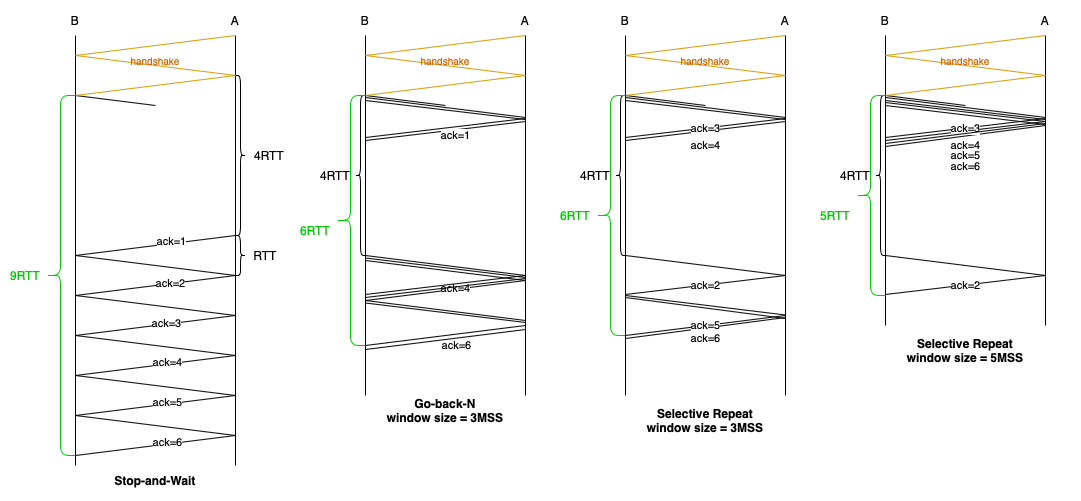
\includegraphics[width=0.95\textwidth]{Solutions/pics/Q5_solution.png}
\caption{نمودار ارسال و تأیید بسته‌ها}
\label{fig:small-example}
\end{figure}
